 \documentclass{article}
    \usepackage{amsmath}
    \usepackage[utf8]{inputenc}
    \usepackage[english]{babel}
    \usepackage{color}
    \usepackage{graphicx}
    \usepackage{enumitem}
    \usepackage{incgraph}
    \hyphenpenalty=10000
    \exhyphenpenalty=10000
    % \usepackage[T1]{fontenc}
    % \usepackage{geometry}
    \usepackage[top = 2cm, bottom = 2cm]{geometry}
    
    \usepackage[familydefault,light]{Chivo} 
    \usepackage[T1]{fontenc}
    
    \setlength{\parindent}{4em}
    \setlength{\parskip}{2em}
\renewcommand{\baselinestretch}{1.5}
    \usepackage{graphicx}
    
    \title{COL 783 \\ Assignment 3}
    \author{Rajbir Malik \\ 2017CS10416}
    
    \begin{document}
    
    \maketitle

%  Starting page
% -------------------------------------------------------
% -------------------------------------------------------
    \begin{center}
    \Large{\underline{\textbf{Pyramids and Wavelets}}}
    \end{center}
    \subsection*{Overview}
    In this assignment, we tried various transforms and transformations on the images, checking their benifits in \textit{denoising} and \textit{compression}.\\ 
    We worked with pyramids, \textit{laplacian} and \textit{gaussian}, we tried blending of images. We, also, used pyramids to denoise various images.\\
    We then worked on \texttt{Haar Transform} and \texttt{Lazy-Lifting Transform}, and used them for denoising and compression. I deviced my own encoding and decoding schemes, which seemed to suit very well.\\
% -------------------------------------------------------
% -------------------------------------------------------
% Topic I
    \pagebreak
    \subsection*{Image Blending Using Pyramids}
% -------------------------------------------------------

    \begin{figure}[!htb]
    %
    \minipage{0.45\textwidth}
    \begin{center}
      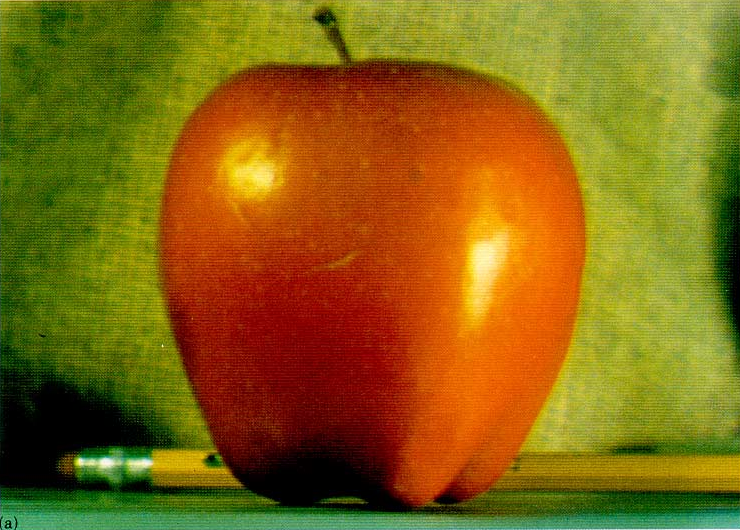
\includegraphics[scale=.35]{./blending/ao/apple.png}
      \caption{Apple}
    \end{center}
    \endminipage \hfill
    %
    \minipage{0.45\textwidth}
    \begin{center}
      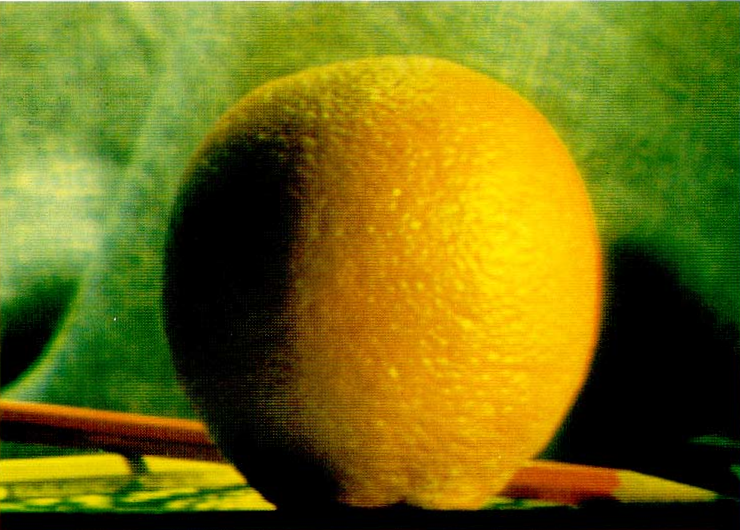
\includegraphics[scale=.35]{./blending/ao/orange.png}
      \caption{Orange}
     \end{center}
    \endminipage \hfill
    %
    \end{figure}

% -------------------------------------------------------
    \phantom{}\\
% -------------------------------------------------------

    \begin{figure}[!htb]
    %
    \minipage{0.35\textwidth}
      \fbox{
\includegraphics[scale=.3]{./blending/ao/1.png}}
      \caption{Merger}
    \endminipage \hfill
    %
    \minipage{0.35\textwidth}
      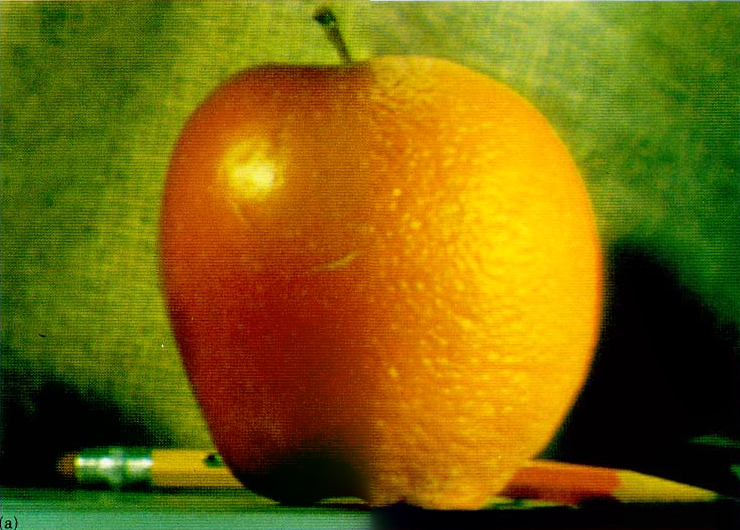
\includegraphics[scale=.3]{./blending/ao/final_1.png}
      \caption{Merge}
    \endminipage \hfill
    %
    \end{figure}
    
% -------------------------------------------------------
    \phantom{}\\
% -------------------------------------------------------
    \pagebreak
% -------------------------------------------------------
    
    \begin{figure}[!htb]
    %
    \minipage{0.35\textwidth}
      \fbox{
\includegraphics[scale=.3]{./blending/ao/2.png}}
      \caption{Merger}
    \endminipage \hfill
    %
    \minipage{0.35\textwidth}
      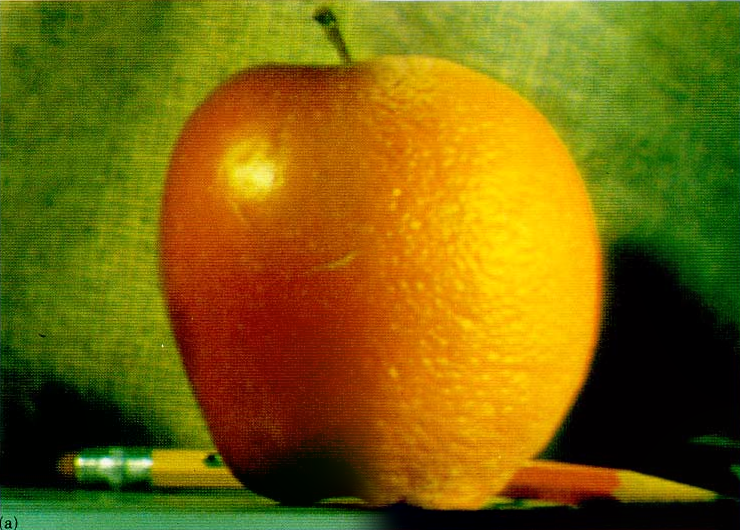
\includegraphics[scale=.3]{./blending/ao/final_2.png}
      \caption{Merge}
    \endminipage \hfill
    %
    \end{figure}

% -------------------------------------------------------
    \phantom{}\\
% -------------------------------------------------------
    
    \begin{figure}[!htb]
    %
    \minipage{0.35\textwidth}
      \fbox{
\includegraphics[scale=.3]{./blending/ao/3.png}}
      \caption{Merger}
    \endminipage \hfill
    %
    \minipage{0.35\textwidth}
      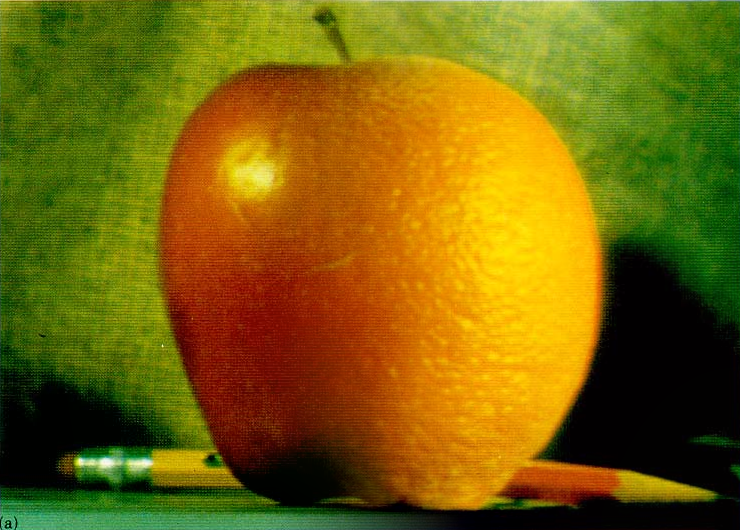
\includegraphics[scale=.3]{./blending/ao/final_3.png}
      \caption{Merge}
    \endminipage \hfill
    %
    \end{figure}
    
    \phantom{}
    
    \pagebreak
    
% -------------------------------------------------------
% Denoising
    \subsection*{Denoising}
    


    \begin{figure}[!htb]
    \minipage{0.45\textwidth}
      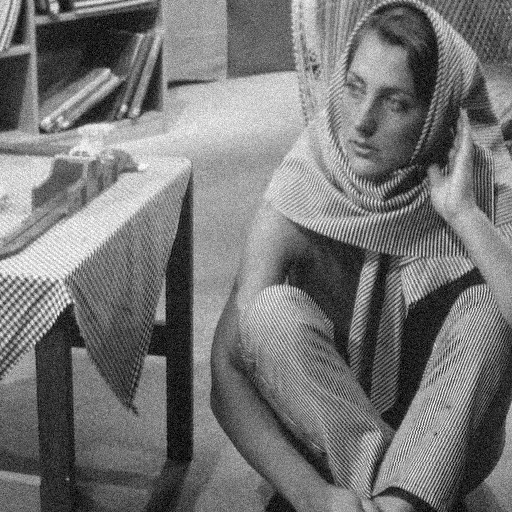
\includegraphics[scale=0.4]{./denoising/b/b05.png}
      \caption{Noisy Image}
    \endminipage \hfill
    \minipage{0.45\textwidth}
      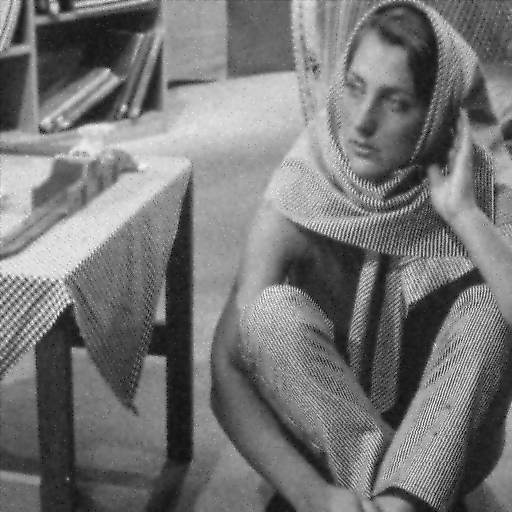
\includegraphics[scale=.4]{./denoising/b/p_1_0.013.png}
      \caption{Pyramid Denoising}
    \endminipage
    \end{figure}
    

    \begin{figure}[!htb]
    \minipage{0.45\textwidth}
      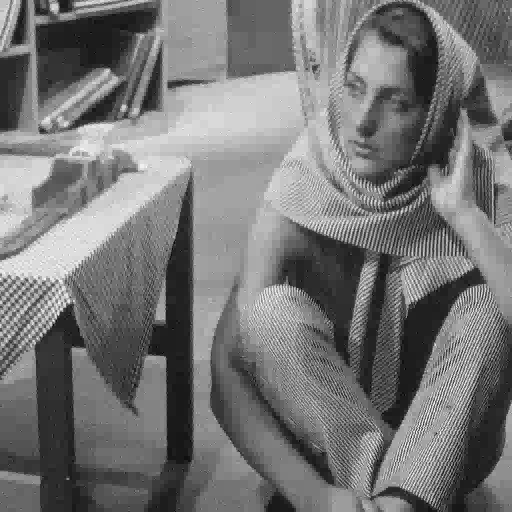
\includegraphics[scale=0.4]{./denoising/b/hard0.15.png}
      \caption{Hard Denoising}
    \endminipage \hfill
    \minipage{0.45\textwidth}
      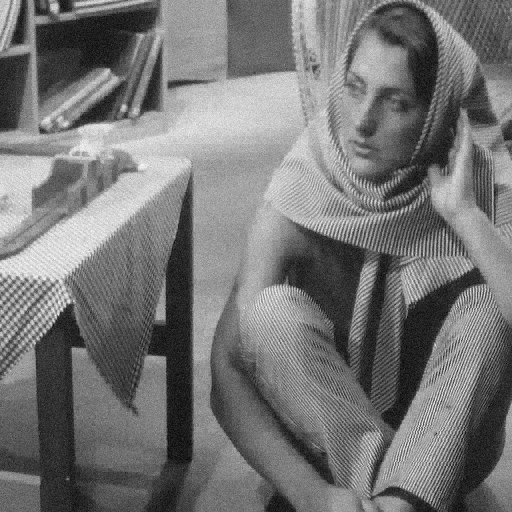
\includegraphics[scale=.4]{./denoising/b/smooth0.05.png}
      \caption{Soft Denoising}
    \endminipage
    \end{figure}
    \pagebreak

%---------------------------------------------    
    \pagebreak

    \begin{figure}[!htb]
    \minipage{0.45\textwidth}
      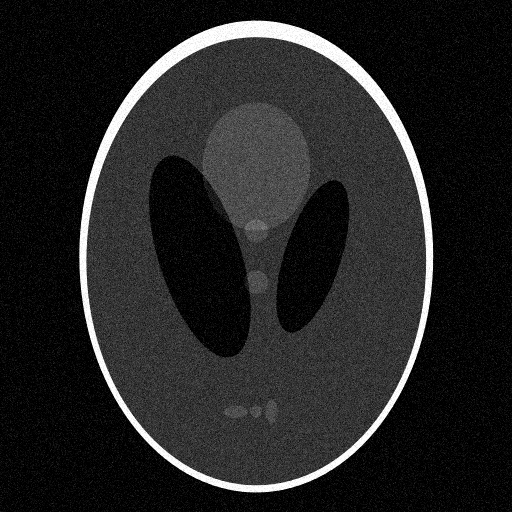
\includegraphics[scale=0.4]{./denoising/n/n05.png}
      \caption{Noisy Image}
    \endminipage \hfill
    \minipage{0.45\textwidth}
      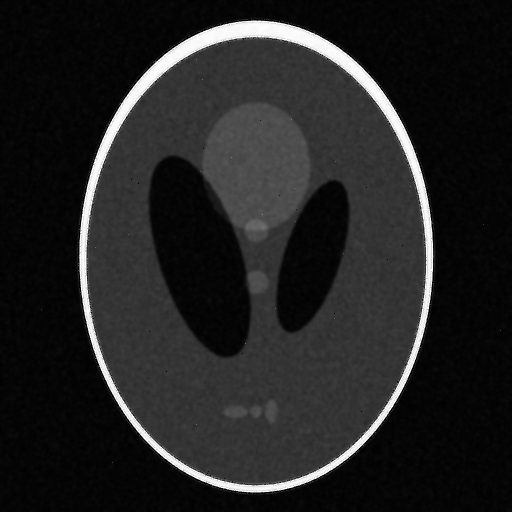
\includegraphics[scale=.4]{./denoising/n/p_1_0.013.png}
      \caption{Pyramid Denoising}
    \endminipage
    \end{figure}
    

    \begin{figure}[!htb]
    \minipage{0.45\textwidth}
      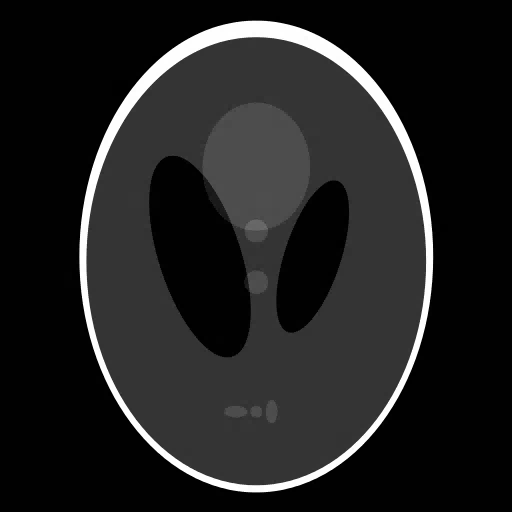
\includegraphics[scale=0.4]{./denoising/n/hard0.05.png}
      \caption{Hard Denoising}
    \endminipage \hfill
    \minipage{0.45\textwidth}
      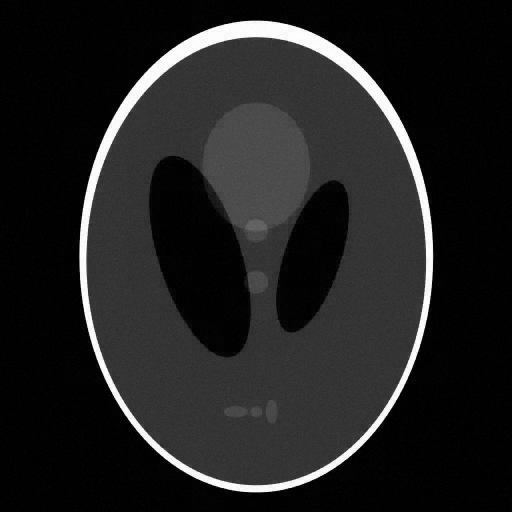
\includegraphics[scale=.4]{./denoising/n/smooth0.05.png}
      \caption{Soft Denoising}
    \endminipage
    \end{figure}
    \pagebreak

%--------------------------------------------- 


\end{document}